\chapter{Experiments}
\label{ch:its-experiments}

Several techniques and algorithms have been combined in the design of the \gls{its}.
With the implementation and evaluation of each of these, new insights were gained into the mental model of the developer. 
In this section, I describe the four experiments I conducted to evaluate and fine-tune each component in the \gls{its}.

\summarybox{
In the first experiment, I evaluated the results of the \gls{2pl} model through statistical analyses.
I found that the assigned difficulty of an exercise on the \gls{scw} platform does not accurately represent the actual difficulty as experienced by the users.
The statistical tests show that the actual difficulty does depend on the framework of the exercise, the category of the vulnerability, and the presentation of the exercise to the user. 

The second experiment showed that out of the tested approximation methods, the one invented in this work is the best to achieve a fast ability estimate at each point in time.
The mean error stays below 10\% even after more than 200 completed challenges.

In the final two experiments, I tested the performance of different \gls{cf} algorithms and their adaptations to learning systems.
The adaptations caused an increase in prediction accuracy between 3.9\% and 13.7\%, depending on the algorithm.
The best performing algorithm in the end is the \gls{knn} baseline algorithm, achieving a mean absolute error of 0.4206.
}

\section{Rash model}
\label{sec:eval-rasch}

\subsection{Goals and research questions}
The main \textit{goal} of the first experiment is to discover correlations between the difficulty of an exercise as estimated by the Rasch model, and characteristics of that exercise.
The \textit{purpose} is to gain insights in the mental model of the developer, and discover which languages, frameworks, or vulnerability types are typically more difficult.
The results of this experiment can be used in the \gls{its} to approximate the difficulty of an exercise when there is no sufficient data available to obtain an estimate with \gls{irt}.

The above goal can be achieved by means of an experiment aimed at answering the following questions:
Is there a statistically significant correlation between the difficulty of a challenge and its
\begin{itemize}
    \item \textbf{Q1} assigned difficulty on the \gls{scw} platform?
    \item \textbf{Q2} vulnerability category?
    \item \textbf{Q3} vulnerability type (subcategory)?
    \item \textbf{Q4} language and framework?
    \item \textbf{Q5} presentation form (locate, identify, fix)?
\end{itemize}

It is expected that the last four characteristics have a significant influence on the difficulty of a challenge.
Some vulnerabilities are more difficult to detect, understand, or fix than others.
This is evident, for example, from the \gls{owasp} Top 10 pages, where each category is assigned a score for exploitability, prevalance, detectability, and technical impact.
There is no clear explanation as to how these scores are determined.
Personal and anecdotal evidence also shows that it is more difficult to get security right while working in certain languages and frameworks.

The first variable, the assigned difficulty on the \gls{scw} platform, is expected to have little impact on the actual difficulty.
As explained in Appendix~\ref{app:challenges}, this difficulty only represents the likelihood of a correct answer in case of a blind guess.
It does not take into account the contents of the exercise, only the number of options to choose from.
While the amount of options is expected to have some influence on the actual difficulty, this effect is likely to be small compared to other characteristics of the exercise.

\subsection{Experimental set-up}
In Section~\ref{sec:calib} it was previously mentioned that calibration techniques for the Rasch model are mostly designed for item banks with several dozens of items.
The larger size of the item bank of \gls{scw} will cause longer execution times and more difficult convergence to stable estimates.
I solved this problem by splitting the item bank into several smaller item banks and calibrating each of them separately.

The downside to this approach is that the Rasch model does not use an absolute scale.
This is evident from the equation for the \gls{1pl} model in Equation~\ref{eq:1pl}, repeated here for convenience in Equation~\ref{eq:1pl-2}.

\begin{equation}
    \label{eq:1pl-2}
    P_{j}(\bm{\theta}_i,\bm{p}_j) =
    Pr(X_{ij} = 1 | \bm{\theta}_i,b_j) =
    \frac{\exp(\theta_i - b_j)}{1 + \exp(\theta_i - b_j)}
\end{equation}

Adding or subtracting the same value from both the difficulty parameter $b_j$ and the ability level $\theta_i$ will cancel out and result in the same probability of a correct answer $P_j$.
In other words, the origin of the scale can be chosen arbitrarily.
In practice, the origin is often set to the mean of the ability estimates~\cite{magis2017computerized}.
I used the R package \texttt{TAM} to estimate the item and person parameters~\cite{robitzsch2021package}.
In the documentation of this package there is no information about the chosen scale.
Based on the implementation that is available on GitHub\footnote{\url{https://github.com/cran/TAM/blob/master/R/tam.mml.2pl.R}}, the scale is set to the mean of the difficulty estimates after the first iteration of the calibration process.
For each item bank that is calibrated separately, the results can hence not be easily compared to other item banks, as they each have their own scale.

However, for this experiment it is necessary to compare the difficulty of challenges across the entire platform.
To be able to do this, the entire item bank has to be calibrated at once. 
The necessary computations took over 73 hours to complete, confirming once more that it would not be feasible to use in the \gls{its}.

\subsubsection{Statistical significance}
With this single Rasch model calibrated, there is a difficulty estimate for every challenge on the platform.
It is now possible to group these challenges according to different characteristics and compute the mean difficulty of each group.
Before we can compare the mean difficulties for each characteristic, however, the results have to be tested for statistical significance.

Which test can be used to do this, depends on the values each characteristic can take.
The difficulty as assigned on the \gls{scw} platform takes on values between 0 and 100, and is hence a numerical variable.
The vulnerability category, vulnerability type, framework, and presentation form are each categorical variables.
Each of these characteristics can only take a limited number of categorical values.

To test the correlation between the difficulty on the \gls{scw} training platform and the \gls{irt} difficulty, the coefficient of determination (R-squared) can be used, as both variables are numerical variables.
The test (R = 0.03, $p = 1.85 \times 10^{-3}$) determines that no significant variation in the \gls{irt} difficulty can be explained by the \gls{scw} difficulty.
This is no surprise, it is clear that the current difficulty assigned on the platform is not an accurate representation of the actual difficulty.

A one-way \gls{anova} can be used for the categorical variables.
This test determines if there is a statistically significant difference between one or more of the possible values that a categorical variable can take.
The one-way \gls{anova} compares the mean difficulty for each of those values and determines whether any of those means are statistically significantly different from each other.
If the one-way \gls{anova} returns a statistically significant result, that means there are at least two values that are statistically different from each other.

The variables were found to have unequal variances across the possible values, a property called heterogeneity of variances.
A Welch \gls{anova} should hence be used, as this \gls{anova} can better control for type I errors~\cite{liu2015comparing}.
The results of the Welch \glspl{anova} are shown in Table~\ref{tab:anova1} and show that a statistically significant difference exists between values for each of the categorical variables.

\begin{table}
    \centering
    \caption[\Gls{anova} test results for Rasch model]{The results of one-way \gls{anova} tests between variables of the exercises and the estimated difficulty. For each variable, the degrees of freedom (df) are shown, as well as the F-statistic, the $p$-value, and the eta-squared ($\eta^2$). All four categorical variables have statistically significant correlations with the estimated difficulty of the exercise. The presentation has a large effect on the estimated difficulty. The category, vulnerability, and framework each have a medium effect.}
    \setcellgapes{4pt}\makegapedcells
    \begin{tabular}{l l S[table-format=3.3] l l}
Variable & df & F & $p$ & $\eta^2$ \\
    \hline
    Category & 36 & 14.154 & $2.97 \times 10^{-53}$ & 0.046 \\
    Vulnerability & 142 & 5.393 & $1.19 \times 10^{-45}$ & 0.079 \\
    Framework & 38 & 11.430 & $ 1.49 \times 10^{-41}$ & 0.060 \\
    Presentation & 3 & 346.164 & $3.00 \times 10^{-6}$ & 0.155 \\
    \end{tabular}
    \label{tab:anova1}
\end{table}

In this \gls{anova} the eta-squared ($\eta^2$) metric was used to measure the effect size of each categorical variable on the estimated \gls{irt} difficulty.
A medium effect was measured for the framework, category, and vulnerability of the exercise and a large effect was measured for the presentation.

Pairwise Games-Howell post-hoc tests were then used to determine which of the values in each categorical variable are statistically different from each other~\cite{games1976pairwise}.
Results of these tests are shown in Table~\ref{tab:gameshowell}.

\begin{table}
    \centering
    \caption[Pairwise Games-Howell post-hoc test results]{The second column displays the number of possible values. Every one of those values is paired with all other values for a pairwise Games-Howell test. The next two columns report the amount of pairs for which the means differ in a statistically significant way, and the amount of pairs for which this is not the case. In the final column the number of values is shown, for which at least one pair exists where the means are statistically significantly different.}
    \setcellgapes{4pt}\makegapedcells
    \renewcommand\theadfont{\normalsize}
    \begin{tabular}{l l l l l}
    Variable & \thead{Values} & \thead{Significant\\ pairs} & \thead{Insignificant\\ pairs} & \thead{Significant\\ values} \\
    \hline
    Category & 36 & 118 & 548 & 29 \\
    Vulnerability & 142 & 384 & 9769 & 77 \\
    Framework & 38 & 217 & 524 & 37 \\
    Presentation & 3 & 3 & 0 & 3 \\
    \end{tabular}
    \label{tab:gameshowell}
\end{table}


With the exception of the presentation, each of the categorical variables has a number of values that do not show a statistical significance with any other value.
If there is no statistical significant difference between two values, this is usually due to insufficient data for one of the values or because the data of one (or both) of the values is too widely spread and there is significant overlap between the data for the two values.
%In the remainder of this section such values are not discussed or shown in any of the graphical displays.
The remaining values show a statistically significant difference in mean difficulty with at least one other value.
When mean difficulties are compared in the remainder of this section, only values are compared whose means show statistically significant differences as determined by the pairwise Games-Howell tests.
Each of the values that are compared explicitly, show statistically significant differences in mean difficulty with a $p$-value of at most 0.05.
The exact $p$-values of these tests are reported in Appendix~\ref{app:pairups}.
%Where appropriate, the $p$-values of the pairwise Games-Howell test for compared categories will be included.

\subsection{Findings}
In this section, I report some of the notable differences in difficulty between different values for each of the characteristics and offer possible explanations for these observations.

\subsubsection{Vulnerability category}
There is a statistically significant difference between the mean difficulty of the four hardest and the four easiest categories.
When comparing these categories to each other, as shown in Figure~\ref{fig:cats1}, their difficulty seems mostly related to the locality of the vulnerability type.

\begin{figure}
    \centering
    %\input{03-education/plots/categories}
    \includegraphics[page=20]{03-education/figures/tikzfigures.pdf}
    \caption[Difficulty of bugs versus flaws]{Vulnerabilities that often require only local changes to the code to fix have lower mean difficulties.}
    \label{fig:cats1}
\end{figure}

The top four categories are (design) \glspl{flaw}, and the fix often involves larger pieces of code.
This is especially the case for business logic flaws and denial of service, where the complexity of the code is the main cause of the problem.
In these categories the developer is unable to foresee unintended results that are a direct result of the logic of their code.
%Some examples are logical errors, uncaught error handling, and problems with regular expressions.

The fixes of the four easiest categories usually only require local changes to the code.
Injection and \gls{xxe} are often fixed by properly sanitizing or whitelisting input parameters, or by configuring components properly.
Security problems related to session management are things like incorrect session lengths, insufficient entropy, or insufficient length for the session \glspl{id}.
Use of vulnerable components is most frequently fixed by updating to a version of the component where the vulnerabilities are fixed.
To fix these vulnerabilities, only local changes to the code are necessary, identifying the correct fix out of several options only involves building a mental model of a small piece of code, making it easier to reason about.

Still, it is noteworthy that the categories near the bottom of the scale are some of the most infamous vulnerabilities.
Injection for example is the top category of the \gls{owasp} top 10 in 2017 and receives high scores for exploitability, detectability, and technicality.
It has currently dropped to the third position in the draft of the next iteration to be released in 2021\footnote{\url{https://owasp.org/Top10/}}.
Based on our training data, at least, it seems that these scores might be exaggerated.
%To explain this, we have to consider the exercises on the \gls{scw} platform.
%To locate a vulnerability in the code, the category of the vulnerability is given.
%At the same time, these vulnerabilities are related to very specific pieces of code. \gls{sql} injection for example can only occur in database queries.
%This makes locating the vulnerability easier.
One exception to this is \gls{xss}.
Despite its infamy, it is closer to the middle of the scale, as can be seen in Figure~\ref{fig:cats2} where \gls{xss} is shown together with all categories it shows statistically significant differences with.
\Gls{xss} being in the middle of the scale can be explained by the fact that there are two major types of \gls{xss}, stored \gls{xss} and reflected \gls{xss}. 
In the case of reflected \gls{xss} the vulnerability is rather local, and the fix is also applied locally, by using output encoding.
For stored \gls{xss} there are usually multiple code fragments involved, one or more where the user input is stored as data and one or more where the stored data is used without output encoding.

In conclusion, the difficulty of the vulnerability correlates to the size of the related code fragments.
Vulnerabilities that only require local changes in the code to fix are easier to understand and fix in training, despite their apparent prevalence in practice.

\begin{figure}
    \centering
    %\input{03-education/plots/categories}
    \includegraphics[page=21]{03-education/figures/tikzfigures.pdf}
    \caption[Medium mean difficulty for XSS challenges]{Challenges about XSS show a mean difficulty around the middle of the scale.}
    \label{fig:cats2}
\end{figure}

\subsubsection{Framework}
Of the 38 different frameworks, 37 show statistically significant differences with at least one other framework.
Pseudocode shows a significant difference with 17 of these frameworks, all of which have a higher mean difficulty.
This makes sense as pseudocode is an artificial language.
It is designed to teach developers algorithms and other programming concepts, and should be easy to understand.

Memory management in memory-unsafe languages such as C and C++ can lead to a whole class of security problems that are avoided in memory-safe languages.
We can see this effect in the higher mean difficulty of C and C++ compared to those of the modern, memory-safe programming languages Java, C\# (.NET), and Python, as shown in Figure~\ref{fig:frames1}.
However, the memory-safe language Cobol also shows a statistically significantly higher mean difficulty compared to each of these three languages.
While Cobol is memory-safe, it does still require memory management and use of pointers, which might explain the higher mean difficulty.
Cobol is also known for its lack of clear documentation regarding security concepts.

\begin{figure}
    \centering
    %\input{03-education/plots/frameworks1}
    \includegraphics[page=9]{03-education/figures/tikzfigures.pdf}
    \caption[Memory-safe versus memory-unsafe languages]{Older programming languages require memory management and use of pointers. They show harder mean difficulties than languages that have automated memory management.}
    \label{fig:frames1}
\end{figure}

Several frameworks show statistically significant differences between the framework and its standard programming language.
This is the case for Java Spring, Java \gls{ee}, Java \gls{jsf}, C\# (.NET) Web Forms, and Python Django.
All of these frameworks are more difficult than their standard language counterparts, as shown in Figure~\ref{fig:frames2}.
This is surprising, as frameworks are designed to implement commonly used functions so that the developer does not have to.
For example, to securely hash a password in standard Java, the developer has to research which algorithm is the most secure, they have to generate a salt using a secure random number generator and correctly combine each of these techniques.
In Java Spring a \texttt{PasswordEncoder} interface is provided, the documentation of this interface is brief and informs developers that \texttt{BCryptPasswordEncoder} is the preferred implementation\footnote{\url{https://docs.spring.io/}}.

Because frameworks often automate these commonly used features, some details of the implementations might be lost to developers.
When the implementation is insufficient, or when the framework is used incorrectly, it is possible that even a security conscious developer can remain unaware of the consequences.
On top of the standard language skills, and the security knowledge, a developer using a framework hence also needs an intimate knowledge of the framework itself to deliver secure code.

\begin{figure}
    \centering
    %\input{03-education/plots/frameworks2}
    \includegraphics[page=10]{03-education/figures/tikzfigures.pdf}
    \caption[Frameworks versus default languages]{All of the frameworks that show statistically significant differences with their standard programming language, have a higher mean difficulty.}
    \label{fig:frames2}
\end{figure}

The mobile framework Java Android is more difficult than web frameworks for the same language (Java \gls{jsf}, Java Spring), as shown in Figure~\ref{fig:frames3}.
This can be explained through the increased attack vectors of mobile applications that are installed on the device of the user.
Because the device and operating system cannot be trusted, the developer has to be aware of other threats, such as restoring backups that are tampered with, detecting root access, and tapjacking.
Unfortunately, Objective C, an extension of C that can be used for mobile development, does not show a statistically significant difference with C itself to confirm this correlation.
The more modern replacement for Objective C, Swift, that is inspired by both C\# (.NET) and Python does show a statistically significant higher mean difficulty than both these languages~\cite{nondot}.

Languages and frameworks have evolved to automate some of the tasks of the developer, such as memory management, and password encryption.
The abstractions provided by these languages and frameworks does not always have a positive impact on security, as is evident from these results.
It is likely that the developers has to sufficiently grasp the implementation details to fully understand the security impact of their code.

\begin{figure}
    \centering
    %\input{03-education/plots/frameworks3}
    \includegraphics[page=11]{03-education/figures/tikzfigures.pdf}
    \caption[Mobile versus web frameworks]{Mobile framework and languages that show statistically significant differences with their web counterparts have higher mean difficulties.}
    \label{fig:frames3}
\end{figure}

\subsubsection{Presentation}
A challenge can be presented to the user as an identify, locate, or fix exercise.
It is unsurprising that identifying a vulnerability that is already marked in the code, is the easiest type of exercise, as shown in Figure~\ref{fig:presentation}. 
On the platform this type of exercise is usually the first stage of a two-stage challenge, with the second stage a fix exercise.

\begin{figure}
    \centering
    %\input{03-education/plots/frameworks3}
    \includegraphics[page=22]{03-education/figures/tikzfigures.pdf}
    \caption[Mean difficulty of challenge presentation]{The mean difficulty of each presentation form is statistically different of the other two. In line with observations in practice, locating a vulnerability in code is the most difficult of the three tasks, followed by fixing the vulnerability.}
    \label{fig:presentation}
\end{figure}

According to the Rasch model, locating vulnerabilities in the code is the most difficult task.
This is in line with observations made in practice, where many vulnerabilities go unnoticed by developers and are detected by automated tools at later stages in the \gls{sdlc}.
\section{Step size adjustment ability estimation}
\label{sec:eval-stepsize}

From the previous experiment in Section~\ref{sec:eval-rasch}, it is evident that calibrating the entire item bank takes a long time.
Similarly, computing the ability estimate based on the entire response pattern of a user takes too long.
Currently, about 15,000 challenges are completed every day, that is about one challenge every five seconds and this number is only expected to go up.
The computations to estimate the ability of a single user easily exceed that.
For a procedure that has to be executed this frequently, even a minute is too long.

\subsection{Goals and research questions}
The main \textit{goal} of this experiment is to evaluate different approximation procedures for the ability estimates.
The \textit{purpose} is to determine if they can be used to improve the efficiency of the ability computations without a significant loss in accuracy.
The \textit{quality focus} is the accuracy of the procedures with increasing numbers of answered items.
The above goal can be achieved by means of an experiment aimed at answering the following question for each procedure:
\begin{itemize}
    \item \textbf{Q1} how big is the mean error of the approximation after every 5 challenges?
\end{itemize}

\subsection{Approximation procedures}
In research literature, I have found two so-called step size adjustment procedures that are used in \glspl{cat}.
These procedures update the latest estimate based on either a fixed or variable step size~\cite{dodd1995computerized}.

\paragraph{Fixed step size} With a fixed step size, the ability estimate is increased (or decreased) by a specific amount, often between 0.4 and 0.7, when the user answers an item correctly (or incorrectly).
In this experiment the smallest step size of 0.4 is used for the evaluation.

\paragraph{Variable step size} With a variable step size the new ability estimate is placed at the halfway point between the current estimate and the difficulty of one of the two most extreme items in the item bank.
This is possible because the calibration techniques of \gls{irt} place users and items on the same scale.
If the user answers an item correctly, then the highest item parameter is used, if not, the lowest is used.
This procedure makes sense when one considers that the item selection algorithm in \glspl{cat} continuously selects items that are significantly above the current estimated ability level of the user, as explained in Section~\ref{sec:cf-alternatives}.
This is not the case for the historical data, and will also not be the case for the item selection of the \gls{its} in the future.
With more forgiving item selection this procedure will likely become inaccurate over time.

\paragraph{Adaptive step size} As an improvement, I have developed a variation of this procedure that uses the difficulty of the selected item instead of the difficulty of the extreme items in the item bank.
This adaptive step size procedure is shown in Algorithm~\ref{al:stepsize}.
When the user answers an item correctly that was expected to be hard, the ability estimate is increased to the halfway point between this item and the current estimate.
Similarly, when the user answers an item incorrectly that was expected to be easy, the ability estimate is decreased to the halfway point.

In the other cases, the outcome of the answer confirms that the current ability estimate is accurate.
A question that is more difficult than the user's current ability level is answered incorrectly, or a question below the ability level is answer correctly.
The player can then optionally be rewarded or punished with a fixed value, similar to the fixed step size adjustment procedure.
For this experiment, two variations of the adaptive step size procedure are tested, one with a fixed reward of 0.2 and one without a fixed reward.

\begin{algorithm}
\SetAlgoLined
\SetKwInOut{Input}{input}
\SetKwInOut{Output}{output}
\Input{user ability $\bm\theta_i$\\ item difficulty $\beta_j$ \\ answer $X_{ij}$ \\an optional punishment/reward value $r$}
\Output{updated user ability $\bm\theta_i$}
    \uIf{$X_{ij}$ is correct}{
        \uIf{$\bm\theta_i \leq \beta_j$}{return ($\bm\theta_i$ + $\beta_j$)/2}
        \Else{return $\bm\theta_i$ + $r$}
    }
    \Else{
        \uIf{$\bm\theta_i \geq \beta_j$}{return ($\bm\theta_i$ + $\beta_j$)/2}
        \Else{return $\bm\theta_i$ - $r$}
    }
\caption{\label{al:stepsize}Adaptive step size adjustment procedure}
\end{algorithm}

\subsection{Experimental set-up}
The different procedures are evaluated by comparing their approximations with the (accurate) estimated \gls{irt} ability.
To do this, an \gls{irt} ability estimate is needed for each user at each point in time, which requires many long-running \gls{irt} calibration procedures.
The five frameworks with the most data were chosen to use in the evaluation.
These are Java Spring, Java \gls{ee}, NodeJS Express, Pseudocode and Python Django.
The \gls{irt} ability was estimated for every user after every 5 completed challenges.

Each of the four procedures starts from the \gls{irt} ability estimate after 20 completed challenges.
From that point forward, the approximation methods are applied to the outcome of each challenge attempt.
The resulting approximations are compared to the \gls{irt} ability after every 5 challenges.

\subsection{Findings}
For each approximation method, the evolution of the mean error as a percent of the full ability scale, is shown Figure~\ref{fig:stepsize}.
The fixed step size adjustment becomes excessively inaccurate after only 15 to 20 challenges following the initial calibration.
After 200 challenges, the mean error of this approximation is up to 300\%.
While the adaptive step size procedure with a fixed reward is significantly better, its error still becomes excessively large and rises indefinitely.
The seemingly ever increasing error for these two procedures is explained by the large amount of users who play challenges that are below their skill level, and hence often answer them correctly.
With these two procedures, the ability level of users like this is increased each time, while these answers have no significant impact on the accurate estimates.

This effect is still visible for the variable step size adjustment procedure.
However, with this procedure the estimate does not exceed the difficulty of the most difficult item in the item bank, which limits the error to about 30\%.

The adaptive step size procedure without reward or punishment is the most accurate.
With this procedure, the ability estimate is not adjusted if the outcome of an item is as expected according to the current estimate.
The ability estimates of users who are answering easy items correctly is not updated.
For correct answers to difficult challenges or for incorrect answers to easy challenges, the estimate is moved in the right direction, but using smaller steps than the variable step size procedure.
The mean error of 10\% is acceptable for it to be used in the \gls{its}, as will become evident in a following experiment in Section~\ref{sec:eval-learning}.
This implies that the full calibration procedure is only necessary once, for the initial calibration.
In practice, the abilities for existing users will still periodically be re-calibrated along with the initial calibration of new users.

\begin{figure}
    \centering
    %\input{03-education/plots/stepsize}
    \includegraphics[page=13]{03-education/figures/tikzfigures.pdf}
    \caption[Error rates of step size adjustment procedures]{The error rates of the two procedures with a fixed step or a fixed reward become excessively large. For the variable step size procedure, the error rate is capped at around 30\%. The adaptive step size procedure without fixed reward is the most accurate and its error rate does not exceed 10\%.}
    \label{fig:stepsize}
\end{figure}

\section{Collaborative filtering algorithms}
\label{sec:eval-cf}

\subsection{Goal and research questions}
The main \textit{goal} of this experiment is to test the prediction accuracy of different (variations of) \gls{cf} algorithms.
The \textit{purpose} is to determine which algorithms are most effective at making recommendations on the \gls{scw} platform.
The \textit{quality focus} is the error of the predicted ratings compared to the observed ratings.
The above goal can be achieved by means of an experiment aimed at answering the following questions:
\begin{itemize}
    \item \textbf{Q1} What is a good error rate for this data set?
    \item \textbf{Q2} Which algorithm achieves the lowest error rate for predicting the utility of an item?
\end{itemize}

\subsection{Benchmark algorithms}
To train and evaluate different (variations of) algorithms, I have used the open-source Python scikit Surprise~\cite{Hug2020}.
Since it is open source, the code is available to download from GitHub and the implemented algorithms can later be adapted to learning systems.

Surprise provides two basic \gls{cf} algorithms that can be used as benchmarks to answer the first research question.

The first benchmark algorithm is called Normal Predictor, it estimates a normal distribution based on the training data and makes new predictions by randomly sampling from this distribution.

The second algorithm is the baseline algorithm.
It uses the baseline estimate as defined in Equation~\ref{eq:baseline-estimate}~\cite{Koren2010}.

\begin{equation}
    \label{eq:baseline-estimate}
    \hat{r}_{ui} = b_{ui} = \mu + b_u + b_i
\end{equation}

In this equation, $\mu$ is the observed overall mean of the ratings, and $b_u$ and $b_i$ are the biases, the average observed deviations of this mean by user $u$ and item $i$.

When computing the utility of an item in Section~\ref{sec:utility} it was observed that some users show a consistent bias.
This is because many users on the \gls{scw} platform stick to the predetermined courses or tournaments.
For users who have a higher ability level, this current selection of challenges is consistently too easy, leading to boredom and hence consistently lower ratings by these users.
The utility experienced by these users can likely be predicted relatively accurately using the baseline algorithm.
Hence it is expected that this benchmark algorithm will already perform well.

\subsection{Memory-based algorithms}
Five memory-based \gls{cf} algorithms are evaluated in this experiment, four \gls{knn} algorithms and an algorithm called the Slope One algorithm.

The \gls{knn} algorithms predict the rating $\hat{r}_{ui}$ of a user $u$ for an item $i$ based on the observed ratings $r_{vi}$ of similar users $v$ for that item.
These algorithms explicitly combine the ratings of the $k$ nearest neighbours to compute a prediction, hence their name as \gls{knn} algorithms.
The difference between these algorithms lies in the exact formulas used to combine the existing ratings of the neighbours to make a prediction.

\paragraph{k-NN basic}
To predict a rating, the first k-NN algorithm, k-NN basic, takes the weighted average of the observed ratings for that item by the $k$ nearest neighbours of the user.
As shown in Equation~\ref{eq:knn-basic}, the similarity between the users is used as the weight in the weighted average.

\begin{equation}
    \label{eq:knn-basic}
    \hat{r}_{ui} = \frac{\sum\limits_{v \in N_i^k(u)} \text{sim}(u, v) \cdot r_{vi} }{\sum\limits_{v \in N_i^k(u)} \text{sim}(u, v)}
\end{equation}

In this equation, $\text{sim}(u,v)$ is the similarity between users $u$ and $v$, and $N_i^k(u)$ is the set of $k$ nearest neighbours of user $u$ that have rated item $i$.
Different similarity metrics can be used, as will be explained later in this section.

The algorithm can also be used to do item-based \gls{cf}, by summing over $j \in N_u^k(i)$, the $k$ nearest neighbours of item $i$ that are rated by user $u$.
In that case, the similarity between items $\text{sim}(i,j)$ needs to be used.

\paragraph{k-NN with means}
The second k-NN algorithm is called k-NN with means.
It does not take the weighted average of the ratings of the nearest neighbours, but instead uses the deviation of the mean, as shown in Equation~\ref{eq:knn-means}.

\begin{equation}
    \label{eq:knn-means}
    \hat{r}_{ui} = \mu_u + \frac{\sum\limits_{v \in N_i^k(u)} \text{sim}(u, v) \cdot (r_{vi} - \mu_v) }{\sum\limits_{v \in N_i^k(u)} \text{sim}(u, v)}
\end{equation}

In this equation, $\mu_u$ is the mean rating given by user $u$.
The algorithm can similarly be used in an item-based fashion.

\paragraph{k-NN with z-score}
The k-NN with z-score algorithm uses the standard score, or z-score of the ratings of each user.
The standard score is the number of standard deviations the rating deviates from the mean.
It can be computed by taking the deviation from the mean, like in the previous equation, and divide the result by the standard deviation.
The resulting formula is shown in Equation~\ref{eq:knn-z-score}.

\begin{equation}
    \label{eq:knn-z-score}
    \hat{r}_{ui} = \mu_u + \sigma_u \frac{\sum\limits_{v \in N_i^k(u)} \text{sim}(u, v) \cdot (r_{vi} - \mu_v) / \sigma_v }{\sum\limits_{v \in N_i^k(u)} \text{sim}(u, v)}
\end{equation}

In this equation, $\sigma_u$ is the standard deviation of the ratings of user $u$.
This algorithm can also be trivially changed to make item-based predictions.

\paragraph{k-NN baseline}
The final k-NN algorithm, k-NN baseline, uses the baselines of the $k$ nearest neighbours to make a prediction, as shown in Equation~\ref{eq:knn-baseline}

\begin{equation}
    \label{eq:knn-baseline}
    \hat{r}_{ui} = b_{ui} + \frac{\sum\limits_{v \in N_i^k(u)} \text{sim}(u, v) \cdot (r_{vi} - b_{vi}) }{\sum\limits_{v \in N_i^k(u)} \text{sim}(u, v)}
\end{equation}

In this equation, $b_{ui}$ is the baseline rating of user $u$ for item $i$, as computed in Equation~\ref{eq:baseline-estimate}.

\paragraph{Similarity metrics}
%Because the \gls{knn} algorithms explicitly make use of the similarity between users (or items) to make predictions, they can be easily adapted to learning systems by adjusting the similarity metric.
The \gls{knn} algorithms described above all make use of the similarity between users (or items) to make predictions, in the formulas this similarity between two users $u$ and $v$ is denoted as $\text{sim}(u,v)$.
Four similarity metrics are considered in this experiment.

The default configurations for the k-NN algorithms use the \textit{\gls{msd} similarity}.
The \gls{msd} is a metric for distance between two users, it sums over all items that have been rated by both users and takes the square of the difference of the given ratings, as shown in Equation~\ref{eq:msd}.

\begin{equation}
    \label{eq:msd}
    \text{msd}(u,v) = \frac{1}
    {\abs{I_{uv}}} \cdot \sum\limits_{i \in I_{uv}} (r_{ui} - r_{vi})^2
\end{equation}

In this equation, $I_{uv}$ is the set of items that have been rated by both users $u$ and $v$.

To use this distance as a similarity measure, the inverse has to be taken.
To avoid dividing by zero, a one is added to the denominator, as shown in Equation~\ref{eq:msd-sim}.

\begin{equation}
    \label{eq:msd-sim}
    \text{msd\_sim}(u,v) = \frac{1}{ \text{msd} (u,v) + 1}
\end{equation}

%To adapt this similarity to learning systems, two attempts have been made.
%First, I have added the difference in ability  as a multiplier to Equation~\ref{eq:msd}.
%As a result, two users will be considered more similar if their ratings are closer together and their abilities were closer together at the time of rating.
%The adapted distance formula is shown in Equation~\ref{eq:msd-adapted}.
%
%\begin{equation}
%    \label{eq:msd-adapted}
%    \text{msd\_adapted}(u,v) = \frac{1}
%    {\abs{I_{uv}}} \cdot \sum\limits_{i \in I_{uv}} (r_{ui} - r_{vi})^2 \cdot \abs{\theta_{ui} - \theta_{vi}}
%\end{equation}
%
%In this equation, $\theta_{ui}$ is the ability level of user $u$ at the time of rating item $i$.
%% not very effective: maybe because similarity in ability level outweighs similarity in rating: what if ratings are far apart, but the users were close in ability level: the difference in rating is canceled out
%% similarity in rating is more important still, similarity in ability level should be a filter rather than a multiplier
%Instead of changing the metric for similarity, the second adaptation instead uses a filter.
%Instead of using all commonly rated items among users to compute the similarity, only items are used for which the similarity is sufficiently close.
%
%\begin{equation}
%    \label{eq:msd-adapted2}
%    \text{msd\_adapted}(u,v) = \frac{1}
%    {\abs{I_{uv}}} \cdot \sum\limits_{i \in I_{uv}} (r_{ui} - r_{vi})^2 \cdot \abs{\theta_{ui} - \theta_{vi}}
%\end{equation}

The second metric, \textit{the cosine similarity}, requires the ratings of the common items between two users to be represented as vectors.
The cosine similarity is then defined as the cosine of the angle between these two vectors, which is the same as the inner product of the two vectors normalized to both have length one.
The resulting formula is shown in Equation~\ref{eq:cosine}.

\begin{equation}
    \label{eq:cosine}
    \text{cosine\_sim}(u,v) = \frac{\sum\limits_{i \in I_{uv}} r_{ui} \cdot r_{vi}}{\sqrt{\sum\limits_{i \in I_{uv}} r_{ui}^2}\cdot\sqrt{\sum\limits_{i \in I_{uv}} r_{vi}^2}}
\end{equation}

The third metric is \textit{the Pearson correlation coefficient}.
It is commonly used in statistics as a measure of correlation between two data sets.
It can be seen as a mean-centered cosine similarity which is evident from similarity of the formula with that of the cosine similarity, as shown in Equation~\ref{eq:pearson}.

\begin{equation}
  \label{eq:pearson}
  \text{pearson\_sim}(u, v) = \frac{ \sum\limits_{i \in I_{uv}}
        (r_{ui} -  \mu_u) \cdot (r_{vi} - \mu_{v})} {\sqrt{\sum\limits_{i
        \in I_{uv}} (r_{ui} -  \mu_u)^2} \cdot \sqrt{\sum\limits_{i \in
        I_{uv}} (r_{vi} -  \mu_{v})^2} }
\end{equation}


\textit{Baseline}, the final similarity metric considered in this experiment, is similar to the Pearson correlation coefficient, but uses baselines for centering instead of means. This similarity metric is shown in Equation~\ref{eq:pearson-baseline}.

\begin{equation}
  \label{eq:pearson-baseline}
        \text{pearson\_baseline\_sim}(u, v) = \frac{
            \sum\limits_{i \in I_{uv}} (r_{ui} -  b_{ui}) \cdot (r_{vi} -
            b_{vi})} {\sqrt{\sum\limits_{i \in I_{uv}} (r_{ui} -  b_{ui})^2}
            \cdot \sqrt{\sum\limits_{i \in I_{uv}} (r_{vi} -  b_{vi})^2}}
\end{equation}

\paragraph{Slope One}
To predict a rating $\hat{r}_{ui}$ of a user $u$ for an item $i$, \gls{knn} algorithms only look at the ratings by similar users for that same item $r_{vi}$.
The ratings of other common items are only used to determine the most like-minded users, not to compute the predicted rating.

In the Slope One algorithm, all ratings of common items are used to make a prediction by computing a popularity differential between each pair of items~\cite{lemire2005slope}.
To compute this popularity differential between two items for two users, the rating of one user for this item is subtracted from the rating of the other~\cite{Hug2020}.
This can be done for all users to receive an average popularity differential between these two items, as shown in Equation~\ref{eq:pop-diff}.

\begin{equation}
  \label{eq:pop-diff}
  \text{popularity\_differential}(i,j) = \frac{1}{\abs{U_{ij}}} \sum\limits_{u \in U_{ij}} r_{ui} - r_{uj}
\end{equation}

In this equation, $U_{ij}$ is the set of all users who rated both items $i$ and $j$.

This popularity differential can then be used to make predictions for the ratings, by taking the mean rating of a user and adding the average popularity differential between two items to this mean, as shown in Equation~\ref{eq:slope-one}.

\begin{equation}
  \label{eq:slope-one}
  \hat{r}_{ui} = \mu_{u} + \frac{1}{\abs{R_{i}(u)}} \sum\limits_{j \in R_{i}(u)} \text{popularity\_differential}(i,j)
\end{equation}

With $R_i(u)$ the set of items $j$ that have been rated by $u$ and also have been rated by at least one other user that has rated $i$.


\subsection{Model-based algorithms}
Besides these memory-based algorithms, Surprise also offers implementations for five popular model-based algorithms~\cite{Hug2020}, one based on clustering and four based on matrix factorization.

\paragraph{Co-Clustering}
The discussed memory-based algorithms make predictions based on a neighbourhood of either like-minded users or similarly-rated items.
In the Co-Clustering \gls{cf} algorithm, the idea is to simultaneously obtain user and item neighbourhoods via co-clustering~\cite{george2005scalable}.
Many algorithms exist to assign these co-clusters, sometimes called biclusters~\cite{tanay2005biclustering}.
The implementation in Surprise is a more straightforward optimization method, similar to k-means~\cite{Hug2020}.

The average ratings from these clusters can then be used to make predictions about the ratings, as shown in Equation~\ref{eq:co-clustering}.

\begin{equation}
  \label{eq:co-clustering}
  \hat{r}_{ui} = \overline{C_{ui}} + (\mu_u - \overline{C_u}) + (\mu_i
        - \overline{C_i})
\end{equation}

In this equation, $\overline{C_{ui}}$ is the average rating of co-cluster $C_{ui}$, $\overline{C_u}$ is the average rating of the cluster of user $u$, and $\overline{C_i}$ is the average rating of the cluster of item $i$.
%The number of user and item clusters can be configured, in this experiment, the default values of 3 item and 3 user clusters are used.

\glsreset{pmf}
\paragraph{\gls{pmf}}
Matrix factorization models map both the users and the items to a space of latent factors of dimensionality $f$.
This latent space tries to explain ratings by characterizing both users and items.
For example, on the \gls{scw} training platform, factors might be obvious characteristics of items such as the vulnerability category, or the presentation of the item.
It is also possible that they represent less defined dimensions such as readability of the code, or the structure of the files, or even completely uninterpretable dimensions~\cite{Ricci2010}.

Each item $i$ is then depicted as a vector $q_i \in \mathbb{R}^f$, that measures the extent to which this item possesses the characteristics represented in the latent space.
Each user $u$ is represented by a vector $p_u \in \mathbb{R}^f$ that measures the extent of the interest (or utility) this user has for the corresponding factors.

The dot product of these two vectors captures the interest (or utility) of the user for this item and can be used to make predictions, resulting in the \gls{pmf} algorithm~\cite{mnih2008probabilistic,Hug2020}.
The formula is shown in Equation~\ref{eq:pmf}.

\begin{equation}
  \label{eq:pmf}
  \hat{r}_{ui} = q_i^T p_u 
\end{equation}

\glsreset{svd}
\paragraph{\gls{svd}}
The \gls{svd} algorithm is similar to \gls{pmf}, but creates a final rating by also adding the baseline predictors~\cite{koren2009matrix, Ricci2010, Hug2020}. 
The resulting formula is shown in Equation~\ref{eq:svd}.

\begin{equation}
  \label{eq:svd}
  \hat{r}_{ui} = \mu + b_u + b_i + q_i^T p_u 
\end{equation}

To estimate each of these unknown variables, the following regularized squared error needs to be minimized:

\begin{equation}
     \sum_{r_{ui} \in R_{train}} \left(r_{ui} - \hat{r}_{ui} \right)^2 +
        \lambda\left(b_i^2 + b_u^2 + ||q_i||^2 + ||p_u||^2\right)
\end{equation}

The constant $\lambda$ controls the extent of regularization, in this experiment it is set to 0.02. Minimization of the error is typically done using stochastic gradient descent~\cite{Hug2020, Ricci2010}.
In this process, the algorithm makes predictions for all existing ratings and computes the prediction error.
All parameters are then moved slightly in the opposite direction to improve the predictions in the next pass.
For the algorithm in this experiment, this process was repeated 20 times to reach the final estimates.

\paragraph{\gls{nmf}}
The \gls{nmf} \gls{cf} algorithm is also similar to \gls{pmf}, but the user and item factors are kept positive~\cite{NMF:2014, NMF_algo, zhang2006learning, Hug2020}.
That means each item $i$ is depicted as a vector $q_i \in \mathbb{R}_{\geq 0}^f$, and each user $u$ as a vector $p_u \in \mathbb{R}_{\geq 0}^f$.
Predictions are then computed identically to \gls{pmf}, as shown in Equation~\ref{eq:pmf}.

To ensure that the parameters remain positive, a stochastic gradient descent is used that ensures non-negativity of factors based on the step size and the initial values~\cite{Hug2020}.

\paragraph{SVD++}
The SVD++ algorithm was developed to make use of implicit feedback.
It builds on the assumption that the users can also be characterized by accounting for which items they have or have not provided a rating for.
The SVD++ algorithm often results in superior accuracy compared to \gls{svd}.

A second set of item factors $y_i \in \mathbb{R}^f$ is added that is used to characterize the users based on the set of items they have rated.
The user vector $p_u$ is then extended based on these characteristics before using it to compute a prediction, as shown in Equation~\ref{eq:svdpp}. 

\begin{equation}
  \label{eq:svdpp}
    \hat{r}_{ui} = \mu + b_u + b_i + q_i^T\left(p_u +
        |I_u|^{-\frac{1}{2}} \sum_{j \in I_u}y_j\right)
\end{equation}

\subsection{Experimental set-up}
To evaluate the various \gls{cf} algorithms in this section, I have selected the five frameworks with the most data available on the platform.
These are Java Spring, Java \gls{ee}, NodeJS Express, Pseudocode and Python Django.
For each of those frameworks, I have iterated over the challenge attempts in the data set and continuously estimated the ability of each user.
This estimate is computed with the adaptive step size adjustment procedure, evaluated in the previous experiment of this chapter.
This ability estimate was then used to rate each challenge attempt according to its utility for the user, as described in Section~\ref{sec:utility}.
The resulting ratings, on a scale of 1 to 5, are used to evaluate the (variations of) \gls{cf} algorithms.

\begin{itemize}
    \item The two benchmark algorithms are tested.
    \item All four \gls{knn} algorithms are tested with default configurations.
    \item Each \gls{knn} algorithm is tested with item-based similarities.
    \item Each of the four \gls{knn} algorithms is tested with all four similarity metrics.
    \item Slope One is tested with default configurations.
    \item All five model-based algorithms are tested with default configurations.
\end{itemize}

Each (variation of an) algorithm is evaluated on each of the five selected frameworks using a process of 10-fold cross-validation.
In this process, the data set of the framework is split into 10 equal parts, called folds.
Next, 9 of the 10 folds are used as training data, and the final fold is used as test data.
Every time an algorithm is evaluated on a fold of test data, this is done with three different evaluation metrics that will be explained further in this section.
This process is repeated 10 times, each time alternating the fold to be used as test data.
So for each algorithm and framework combination, 10 measurements are obtained, one for each fold.
The final step of the cross-validation process is to take the mean and standard deviation of these 10 measurements.

The mean of the 10 measurements is used to evaluate the algorithm on this particular data set, as it represents the mean performance of the algorithm.
I will call this the framework-mean $\mu_f$ for an algorithm.
The set of five framework-means for an algorithm is then denoted as $M_f$.
The standard deviation can be used to assess the algorithm for overfitting.
Overfitting is a prediction error caused when the algorithm is too closely aligned to the training sets, causing decreased performance on (some of) the test sets.
Analogous with the framework-mean, this will be denoted as $\sigma_f \in S_f$.

If all five standard deviations $\sigma_f \in S_f$ are sufficiently small, we can take the mean of the five framework-means $\mu_f \in M_f$ to obtain a final result that enables us to evaluate the algorithm's performance on all five frameworks.
This mean will be called the algorithm-mean $\mu_{a}$.
In Appendix~\ref{app:its-metrics}, the algorithm-mean is reported for every (variation of) algorithm evaluated, as well as the largest of the framework standard deviations $\sigma_{max} = \text{max}(\sigma_f \in S_f)$ to show that no overfitting is taking place.

\subsubsection{Metrics}
% https://surprise.readthedocs.io/en/stable/accuracy.html
To evaluate the \gls{cf} algorithms, I have used three metrics that compare the set of predicted ratings $\hat{R}$ to the set of observed ratings $R$.

\paragraph{\gls{mae}}
One of the most popular metrics in research literature is the \gls{mae}~\cite{sarwar2001item,su2009survey}.
It computes the average prediction error over the entire set of predictions, as shown in Equation~\ref{eq:mae}.
\begin{equation}
    \label{eq:mae}
    \text{MAE} = \frac{1}{ |\hat{R}| }  \sum\limits_{\hat{r}_{ui} \in \hat{R}} |r_{ui} - \hat{r}_{ui}|
\end{equation}

The \gls{mae} uses the same scale as the ratings itself, and hence cannot be used to make comparisons between measurements using different scales.
For this the \gls{nmae} can be used that expresses the error as a percentage of the full scale~\cite{su2009survey}.
In our rating scale, the \gls{mae} takes values between 0 for a perfect prediction and 5 as the maximum error.

\paragraph{\gls{rmse}}
The \gls{rmse} amplifies the error between the actual rating and the predictions by taking the square of the prediction error, as shown in Equation~\ref{eq:rsme}.

\begin{equation}
    \label{eq:rsme}
    \text{RMSE} = \sqrt{ \frac{1}{ |\hat{R}| }  \sum\limits_{\hat{r}_{ui} \in \hat{R}} (r_{ui} - \hat{r}_{ui})^2}
\end{equation}

Like the \gls{mae}, the \gls{rmse} is scale-dependent.
It takes non-negative values and a lower value means better prediction performance.

The \gls{rmse} has increased in popularity, partly because of its use in the Netflix competition for movie recommendations~\cite{su2009survey,zhou2008large}.
In 2006, Netflix launched a competition to beat the current score of their recommendation algorithm, \emph{Cinematch}.
At the time the algorithm achieved a \gls{rmse} of 0.9514~\cite{zhou2008large,bennett2007netflix}.
With the competition, Netflix offered a \$1 million dollar prize to the team that could improve this benchmark by 10\%.
The algorithm of the winners, one year later, reached a \gls{rmse} of 0.8567 and was put into production~\cite{zhou2008large,netflixprizeforum,netflixprizeleaderboard}.
This also shows that in \gls{cf} algorithms, improvements of several percents can already be valuable.

\paragraph{\gls{fcp}}
Finally, I have also included a measure that puts more focus on the order the items are ranked rather than the exact rating that is predicted.
In the \gls{fcp}, the number of concordant pairs $n_{c}^{u}$ for a user $u$ is determined by counting the pairs of ratings that are ranked correctly~\cite{koren2013collaborative}.
This is shown in Equation~\ref{eq:concordantpairs}.

\begin{equation}
    \label{eq:concordantpairs}
    n_{c}^{u} = |\{(i,j) \mid \hat{r}_{ui} > \hat{r}_{uj} \text{ and } r_{ui} > r_{uj} \}|
\end{equation}

The number of pairs that is ranked incorrectly is the number of discordant pairs $n_{d}^u$.

The total number of concordant pairs $n_c$ and discordant pairs $n_d$ is then obtained by summing over all users, as shown in Equation~\ref{eq:concordant2}.

\begin{equation}
    \label{eq:concordant2}
    n_{c} = \sum\limits_{u} n_{c}^{u},\qquad n_{d} = \sum\limits_{u} n_{d}^{u}
\end{equation}

Using this total number of concordant and discordant pairs, the FCP can be computed as shown in Equation~\ref{eq:fcp}.

\begin{equation}
    \label{eq:fcp}
    \text{FCP} = \frac{n_{c}}{n_{c} + n_{d}}
\end{equation}

The \gls{fcp} takes values between 1 and 0, with higher meaning that a larger portion of pairs are ranked correctly.


\subsection{Findings}
All measurements during this experiment are included in the tables of Appendix~\ref{app:its-metrics}.
In this section, I will discuss some interesting results, and mainly use the \gls{mae} to compare the performance of algorithms.

\subsubsection{Benchmark}
The benchmark algorithms perform reasonably well.
The Baseline algorithm in particular, as it reaches a $\mu_a$ \gls{mae} of 0.5004 and $\mu_a$ \gls{rmse} of 0.6169.
This is significantly lower than the prediction error for the Netflix prize for example, where the winner reached a \gls{rmse} of 0.8567~\cite{zhou2008large,netflixprizeforum,netflixprizeleaderboard}. 
The Netflix recommendations happen to use the same scale as the utility rating in this experiment, so this comparison can be made.
These results indicate that the utility of an item on the \gls{scw} platform is in comparison easier to predict.

The good performance of the Baseline algorithm was expected based on the observations of the data.
In the current item selection, most users are given the same exercises.
These items are of course not randomly selected, but carefully tailored by the \gls{scw} employees who designed these \gls{owasp} Top 10 courses on the platform.
As a result, for a number of users this item selection is rather good, and the ratings of these users are consistently high.
For more experienced users, the content of these courses is too easy, and as a result their ratings are consistently lower.
Using baselines, these consistent bias result in reasonably accurate predictions.

\subsubsection{Memory-based algorithms}
The default configurations of all memory-based algorithms result in improved prediction performance compared to the baseline benchmark.
The Slope One algorithm performs worse than the \gls{knn} algorithms.
It reaches a \gls{mae} of 0.4928 which is an improvement of about 1.5\% compared to the baseline benchmark.
The best performing \gls{knn} algorithm is the \gls{knn} baseline.
As explained before, it is not surprising that baseline algorithms are performing well on this data set.
It reaches a \gls{mae} of 0.4680, improving the baseline benchmark by 6.5\%.


In the next test, the \gls{knn} algorithms were configured to use item-based similarities to find the $k$ nearest neighbouring items, and make predictions based on the ratings of those items.
This item-based configuration performed worse for all four algorithms, with an increase in prediction error between 1.0\% and 6.7\% depending on the algorithm.

In the final test with the \gls{knn} algorithms, each of the algorithms is evaluated in combination with each of the four similarity metrics.
%1 - (0.4840/0.4508) --> over 7\% for k-NN with z-score Cosine and Baseline
The results indicate that the similarity metric can have a big impact on the prediction performance, with as much as a 7\% increase in performance for the \gls{knn} with z-score algorithm between the cosine similarity metric and the baseline similarity metric.

When the similarity metrics are ranked from best to worst performance, this ranking is the same for each algorithm, and is as follows:
\begin{enumerate}[noitemsep]
    \item Baseline similarity,
    \item Cosine similarity,
    \item \gls{msd} similarity,
    \item Pearson similarity.
\end{enumerate}

Once again, the choice based on baselines is the best performing.

For each of the \gls{knn} algorithms, the item-based similarity, computed with the baseline similarity metric, results in the best performance.
The \gls{mae} of the best performing configuration for each memory-based algorithm is shown in Table~\ref{tab:memory-based}, all other measurements are available in Appendix~\ref{app:its-metrics}.

\begin{table}
    \centering
    \caption[Prediction performance of memory-based algorithms]{All memory-based algorithms perform better than the benchmarks. \gls{knn} basic and Slope One perform significantly worse than the other algorithms.}
    \label{tab:memory-based}
    \small
    \begin{tabular}{l ll}
                 & \multicolumn{2}{c}{MAE}\\
    \cline{2-3} 
    & $\mu_a$ & $\sigma_{max}$\\
    \hline
k-NN basic        & 0.4902 & 0.003 \\ 
k-NN with means   & 0.4521 & 0.002 \\ 
k-NN with z-score & 0.4508 & 0.002 \\ 
k-NN baseline     & 0.4514 & 0.002 \\ 
Slope One         & 0.4928 & 0.002 \\
    \end{tabular}
\end{table}

\subsubsection{Model-based algorithms}
In the next test, these results are compared to those of the model-based algorithms, which tend to be more accurate, especially for sparse data.

Surprisingly, none of the model-based algorithms was able to improve the prediction rate of the best performing memory-based algorithm.
Changing parameters in the model-based algorithms had influence on the speed of convergence, but no real impact on the prediction accuracy.
The \gls{mae} for each algorithm is shown in Table~\ref{tab:model-based}, for other measurements consult Appendix~\ref{app:its-metrics}.

SVD++, the best performing of the model-based algorithms, reaches a \gls{mae} of 0.4591, beating the default configurations of all memory-based algorithms.
This is not surprising, as SVD++ also takes into account which items users have and have not rated.
This algorithm can hence make a better distinction between users who followed the standard courses, and users who did not.

Co-Clustering performs the worst of the model-based algorithms and its \gls{mae} is not significantly better than that of the baseline benchmark.
One of the strengths of the Co-Clustering algorithm is that it can handle synonyms rather well.
In recommendation systems, synonyms are items that are (nearly) identical but are still labeled as different items.
Movie databases often have genres like ``Children's movie" and ``Children's film", which are then clustered together by the algorithm.
More data can then be used to make recommendations about either of those genres.
Evidently, on our platform few such synonyms are present, even though for each framework many exercises exist about the same vulnerability types.
The ratings for these exercises are sufficiently inconsistent so that the Co-Clustering algorithm does not result in significant improvements in prediction accuracy.

While model-based algorithms are usually more accurate, this is not the case for the \gls{scw} training data.
This is likely because the advantages of model-based algorithms are not very applicable to this data set, as will be explained in the discussions in Chapter~\ref{ch:its-evaluation}.

\begin{table}
    \centering
    \caption[Prediction performance of model-based algorithms]{Most model-based algorithms perform worse than the fine-tuned memory-based algorithms. SVD++ is the exception, it reaches prediction accuracy close to that of the best performing memory-based algorithms.}
    \label{tab:model-based}
    \small
    \begin{tabular}{l ll}
                 & \multicolumn{2}{c}{MAE}\\
    \cline{2-3} 
    & $\mu_a$ & $\sigma_{max}$\\
    \hline
Co-Clustering     & 0.4999 & 0.007 \\
PMF               & 0.4783 & 0.003 \\
NMF               & 0.4835 & 0.002 \\
SVD               & 0.4750 & 0.003 \\
SVD++             & 0.4591 & 0.003 \\
    \end{tabular}
\end{table}
\section{Adaptation to learning systems}
\label{sec:eval-learning}

Through the above experiments, I am able to obtain an accurate difficulty measure for each challenge, and a good approximation of the ability level of each user at every point in time.
I have also rigorously tested the performance of several \gls{cf} algorithms on the data set.
In the experiment of this section, I will use the ability level of the users to improve the performance of these algorithms.

\subsection{Goals and research questions}
The main \textit{goal} of this experiment is to test the prediction accuracy of different \gls{cf} algorithms after they have been adapted to learning systems.
The \textit{purpose} is to determine if the proposed adaptations in this work lead to improved performance in some or all algorithms.
The \textit{quality focus} is the prediction error of the adapted algorithms in comparison to those of the unaltered algorithms.
The above goal can be achieved by means of an experiment aimed at answering the following question for each algorithm:
\begin{itemize}
    \item \textbf{Q1} Does the error rate of the prediction decrease when the proposed adaptation to learning systems is applied?
\end{itemize}

\subsection{Experimental set-up}
The best performing configuration of each algorithm tested in the previous experiment of Section~\ref{sec:eval-cf} has been adapted to learning systems and measured in this experiment.

The same process of evaluation is used as in the previous experiment, where each algorithm is tested using 10 fold cross-validation on each of the top five frameworks.
For each algorithm, the algorithm mean $\mu_a$ and the largest standard deviation $\sigma_{max}$ of each of the three metrics are reported in Appendix~\ref{app:its-metrics}.

\subsection{Adaptation to learning systems}
The goal of the adaptation is to include the ability level $\theta_{ui}$ of user $u$ at the time of rating item $i$ in the algorithm.
In particular, this ability level should be used to update the similarity between users.
Currently, two users are considered like-minded if they rate common items similarly.
With this adaptation, the goal is to consider two users like-minded if the items they rated around the same ability level are rated similarly.

\subsubsection{Similarity metrics}
The most obvious way to include this ability level is to update the similarity metrics used by the \gls{knn} algorithms.

%\todo[inline]{Should this be included or not?}
%In the first attempt, the most simple similarity metric, the \gls{msd} was changed.
%This similarity metric uses a distance measure.
%In this measure the difference in ability level was added as a multiplier, as shown in Equation~\ref{eq:msd-adapted}.
%The rationale behind this change is that the distance between users would be amplified if the difference in ability levels is large, and conversely, the distance between users would be decreased if the ability levels were close together.
%
%\begin{equation}
%    \label{eq:msd-adapted}
%    \text{msd\_adapted}(u,v) = \frac{1}
%    {\abs{I_{uv}}} \cdot \sum\limits_{i \in I_{uv}} (r_{ui} - r_{vi})^2 \cdot \abs{\theta_{ui} - \theta_{vi}}
%\end{equation}
%
%Testing this change, however, resulted in decreased performance, best explained through two scenarios.
%First, when users have very different ratings for an item, but they were given at nearly the same ability level, these users are still considered similar users due to the multiplicative effect.
%It is easy to see how this is detrimental for the performance of the algorithm.
%Second, when ratings are very close together, but around widely different ability levels, again due to the multiplicative effect, users are still considered similar.
%This is of course the opposite of the intended effect, where the goal was to consider those users dissimilar due to the difference in ability level.
%
%Instead a different adaptation is made to this metric, and all other metrics.

In each of the metrics, to determine the similarity between users $u$ and $v$, summations are made over $I_{uv}$, the items that have been rated by both users $u$ and $v$.
In the adaptation, this set is replaced by $I_{uv}^t$, the items that have been rated by both users $u$ and $v$ and for which the difference in ability level $\delta\theta = \abs{\theta_{ui} - \theta_{vi}}$ at the moment of rating is smaller than the threshold $t$.

In Equation~\ref{eq:baseline-adapted}, this adaptation is demonstrated for the Baseline similarity, the similarity metric that resulted in the best performance in the previous experiment.

\begin{equation}
  \label{eq:baseline-adapted}
        \text{baseline\_adapted\_sim}(u, v) = \frac{
            \sum\limits_{i \in I_{uv}^t} (r_{ui} -  b_{ui}) \cdot (r_{vi} -
            b_{vi})} {\sqrt{\sum\limits_{i \in I_{uv}^t} (r_{ui} -  b_{ui})^2}
            \cdot \sqrt{\sum\limits_{i \in I_{uv}^t} (r_{vi} -  b_{vi})^2}}
\end{equation}

The value of the threshold parameter $t$ needs to be large enough so that there is still enough data within this range to compare users with.
The best performance was measured when $t$ was around a third of the entire ability scale.

\subsubsection{Data processing}
The other algorithms do not explicitly use similarity between the users.
They can still be influenced to take the ability level at the time of rating into account by processing the data first.

Instead of using a filter at the time of computing the similarity, it is possible to filter at the time the rating is given.
To do this, the ability scale is split into three intervals, called expert, intermediate, and novice ability level.

The ability level of the user at the time of rating an item $i$ is taken into account, by splitting the item into three distinct items, $i_{expert}$, $i_{intermediate}$, and $i_{novice}$.
If the user rates the item $i$, the data is then processed as rating one of these three items, based on the ability level of the user at the time of rating.
This processed data can then be used to train the unaltered algorithms.

This is less accurate than adapting the similarity metrics. It is possible that users at the bottom of the expert ability level assign very similar ratings to the users at the top of the intermediate ability level. 
By using a threshold at the time of computing the similarity, these users are still considered similar.
By splitting the ability scale into ranks, they are not.

\subsection{Findings}
The proposed adaptation resulted in improved performance for all of the algorithms, as shown in Table~\ref{tab:improvement}.
The improvement is larger for the \gls{knn} algorithms, because these algorithms make more explicit use of the ratings of neighbours to make a prediction.
The improvement is particularly large for the \gls{knn} basic algorithm, with a 13.7\% decrease in \gls{mae}.
This algorithm is very straightforward and takes the mean of the ratings of the most similar users to make a prediction.
The improvement of this algorithm is a clear indication that the ability level of a user at the time of rating an item has a significant impact on the rating.

The smallest improvement is made by the Co-Clustering algorithm.
This algorithm was already the worst-performing, and it is likely that the effect of splitting the items is somewhat negated by the clustering.

The best performing algorithm after the adaptation is the \gls{knn} baseline, it reaches a \gls{mae} of 0.4206, a total improvement of 16.0\% over the initial baseline benchmark.

\begin{table}
    \centering
    \caption[Adapted collaborative filtering algorithms]{All algorithms have improved performance because of the adaptation to learning systems.}
    \label{tab:improvement}
    %               1 23 4 56 7 89 
    \small
    \begin{tabular}{l ll S[table-format=2.1]}
                 & \multicolumn{2}{c}{MAE} \\
    \cline{2-3}
    & $\mu_a$ & $\sigma_{max}$\\
    \hline
    &\multicolumn{3}{c}{\textsf{Similarity metric}}\\
    \hline
    k-NN basic & 0.4232 & 0.002 & \textcolor{scw-teal-darker}{-13.7\%}  \\
    k-NN with means  & 0.4261 & 0.002 & \textcolor{scw-teal-darker}{-5.7\%} \\
    k-NN with z-score  & 0.4276 & 0.002& \textcolor{scw-teal-darker}{-5.1\%} \\
    k-NN baseline & {0.4206} & 0.003& \textcolor{scw-teal-darker}{-6.8\%} \\
    \hline
    &\multicolumn{3}{c}{\textsf{Data processing}}\\
    \hline
    Slope One     & 0.4719 & 0.002 & \textcolor{scw-teal-darker}{-4.2\%}\\
    Co-clustering & 0.4940 & 0.007
              & \textcolor{scw-teal-darker}{-1.2\%} \\
    PMF & 0.4598 & 0.003 
              & \textcolor{scw-teal-darker}{-3.9\%} \\
    NMF & 0.4614 & 0.003 
              & \textcolor{scw-teal-darker}{-4.6\%}\\
    SVD & 0.4555 & 0.002 
              & \textcolor{scw-teal-darker}{-4.1\%}\\
    SVD++ & 0.4409 & 0.003
              & \textcolor{scw-teal-darker}{-4.0\%} \\
    \end{tabular}
\end{table}

